\section{Projet 7 — Le morpion}

\subsection*{Objectif du jeu}
Réaliser un morpion (3×3) jouable à deux joueurs au clavier, avec affichage ASCII et détection de victoire/égalité.

\subsection*{Règles du jeu}
\begin{itemize}
  \item Affichage de la grille dans le terminal avec des caractères de base : \texttt{'X'} pour le joueur 1, \texttt{'O'} pour le joueur 2.
  \item Les joueurs jouent à tour de rôle tant que 3 caractères ne sont pas alignés. C'est le programme qui vérifie les alignements.
  \item Si un joueur joue sur une case inexistante ou déjà occupée, il \textbf{perd son tour}.
  \item Le jeu se joue avec le \textbf{pavé numérique} du clavier.
  \item En mémoire, la grille est un tableau de \textbf{9 entiers} : \texttt{0} = case vide, \texttt{1} = 'X' (J1), \texttt{2} = 'O' (J2).
\end{itemize}

\begin{center}
  \begin{minipage}{0.45\textwidth}
    \centering
    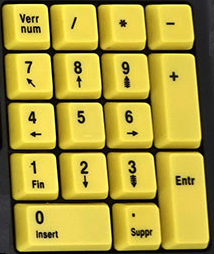
\includegraphics[width=0.8\textwidth]{sources/images/clavier_pave_numerique.png}\\
    \textit{Clavier pour jouer}
  \end{minipage}
  \hfill
  \begin{minipage}{0.45\textwidth}
    \centering
    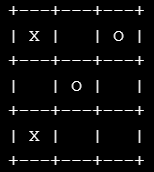
\includegraphics[width=0.6\textwidth]{sources/images/morpion_grille_exemple.png}\\
    \textit{Grille correspondant à \texttt{\{1,0,0,0,2,0,1,0,2\}}}
  \end{minipage}
\end{center}

\subsection*{Correspondance pavé numérique / grille}
Les touches du pavé numérique ont la \textbf{même disposition} que les cases de la grille : appuyer sur une touche désigne la case située au même endroit (la touche \texttt{7} est le coin haut-gauche, la touche \texttt{5} le centre, la touche \texttt{3} le coin bas-droit).

\begin{center}
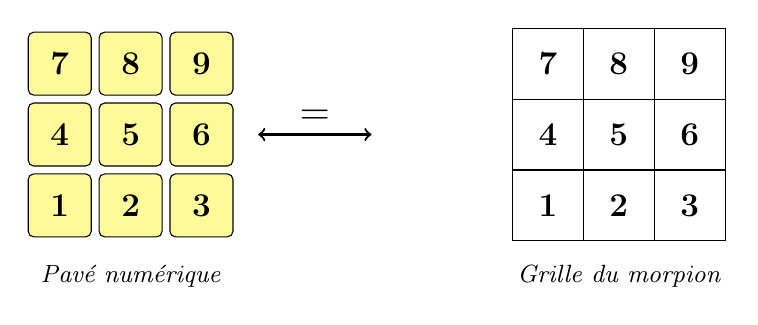
\begin{tikzpicture}[x=0.9cm,y=0.9cm,
  touche/.style={draw,rounded corners=2pt,fill=yellow!40,minimum size=0.8cm,font=\bfseries\large},
  case/.style={draw,minimum size=0.9cm,font=\bfseries\large,fill=white}]
  % pavé numérique
  \foreach \n [count=\i from 0] in {7,8,9,4,5,6,1,2,3} {
    \pgfmathtruncatemacro{\c}{mod(\i,3)}
    \pgfmathtruncatemacro{\l}{int(\i/3)}
    \node[touche] at (\c,-\l) {\n};
  }
  \node[font=\itshape\small] at (1,-3) {Pavé numérique};
  \draw[<->,thick] (2.8,-1) -- (4.4,-1) node[midway,above,font=\Large] {$=$};
  % grille
  \begin{scope}[xshift=6.2cm]
  \foreach \n [count=\i from 0] in {7,8,9,4,5,6,1,2,3} {
    \pgfmathtruncatemacro{\c}{mod(\i,3)}
    \pgfmathtruncatemacro{\l}{int(\i/3)}
    \node[case] at (\c,-\l) {\n};
  }
  \node[font=\itshape\small] at (1,-3) {Grille du morpion};
  \end{scope}
\end{tikzpicture}
\end{center}

\textit{Attention :} en mémoire, la grille est un tableau à 9 cases, indicées de \texttt{0} à \texttt{8} \textbf{ligne par ligne}, du haut vers le bas. L'indice \texttt{0} correspond donc à la touche \texttt{7}, l'indice \texttt{1} à la touche \texttt{8}, \dots{} et l'indice \texttt{8} à la touche \texttt{3} : à vous de convertir la touche saisie en indice du tableau.

\begin{center}
\begin{tabular}{|l|*{9}{c|}}
\hline
Indice du tableau & 0 & 1 & 2 & 3 & 4 & 5 & 6 & 7 & 8 \\ \hline
Touche à saisir   & 7 & \dots & \dots & \dots & \dots & \dots & \dots & \dots & \dots \\ \hline
\end{tabular}
\end{center}

Pour tester, déclarez le tableau et initialisez-le avec ces valeurs, puis affichez la grille pour vérifier (voir aide).

\subsection*{Cahier des charges}
\begin{UPSTICahierDesCharges}{1}
\begin{itemize}
  \item Boucle infinie munie d'un compteur de passages : si le compteur est pair, afficher \og joueur 1 joue \fg{}, sinon \og joueur 2 joue \fg{}. \textbf{Même code} pour les deux joueurs (c'est la variable \texttt{l\_joueur} qui fait la différence).
  \item Saisie de la case par le joueur \textbf{sans vérification} : affecter la case correspondante avec 1 (J1) ou 2 (J2).
  \item Afficher la grille après chaque coup.
\end{itemize}
\end{UPSTICahierDesCharges}

\begin{UPSTICahierDesCharges}{2}
\begin{itemize}
  \item Si la case n'existe pas ou est déjà occupée, le joueur \textbf{perd son tour} : la case n'est pas affectée et on passe au joueur suivant.
  \item \textbf{Détecter} la victoire : le joueur 1 gagne lorsque le \textbf{produit} des 3 cases d'une ligne, d'une colonne ou d'une diagonale vaut 1 ; le joueur 2 lorsqu'il vaut 8.
  \item \textbf{Détecter} la fin de partie sans vainqueur : le produit de toutes les cases est non nul.
\end{itemize}
\textit{Aide :} pensez à utiliser une ou plusieurs boucles \texttt{for} pour les tests.
\end{UPSTICahierDesCharges}

\begin{UPSTICahierDesCharges}{3}
\begin{itemize}
  \item Jouer contre l'ordinateur, muni d'une \textbf{intelligence artificielle} pour ne pas perdre et essayer de gagner.
  \item Écrire une fonction prenant en entrée le tableau de jeu et retournant 1 si le joueur 1 a gagné, 2 si le joueur 2 a gagné, -1 sinon. Demandez de l'aide à votre enseignant.
\end{itemize}
\end{UPSTICahierDesCharges}

